\documentclass[tikz,border=4pt]{standalone}
\usepackage{amsmath,amssymb}
\usetikzlibrary{arrows.meta,positioning,calc,fit,backgrounds}

\definecolor{boxblue}{RGB}{230,239,255}
\definecolor{boxgreen}{RGB}{232,246,236}
\definecolor{boxgold}{RGB}{255,247,223}
\definecolor{boxrose}{RGB}{251,236,240}
\definecolor{linegray}{RGB}{72,72,72}
\definecolor{scopegreen}{RGB}{65,140,86}
\definecolor{scopegold}{RGB}{183,138,33}
\definecolor{scopeblue}{RGB}{76,104,180}

\tikzset{
  >={Latex[length=2.6mm,width=1.75mm]},
  flow/.style={-{Latex[length=2.6mm,width=1.75mm]}, line width=1.0pt, draw=linegray, line cap=round, line join=round, shorten >=1pt, shorten <=1pt},
  sideflow/.style={-{Latex[length=2.4mm,width=1.65mm]}, line width=0.95pt, draw=linegray!95, line cap=round, line join=round, shorten >=1pt, shorten <=1pt},
  stage/.style={shape=rectangle, rounded corners=3pt, align=center, draw=linegray, thick, text width=40mm, minimum height=10.4mm, inner sep=3.1pt, font=\footnotesize, fill=boxblue},
  compute/.style={stage, text width=42mm, minimum height=12mm, fill=boxgreen},
  score/.style={stage, text width=45mm, minimum height=14.5mm, fill=boxgold},
  output/.style={stage, text width=27mm, minimum height=10.8mm, fill=boxrose},
  noteheader/.style={rounded corners=2pt, fill=white, draw=#1, text=#1!80!black, font=\scriptsize\bfseries, align=center, inner xsep=3.7pt, inner ysep=2pt, text width=24mm},
  mainscope/.style={draw=scopeblue!78, dashed, rounded corners=3.5pt, inner sep=5.5pt, line width=0.95pt},
  fastscope/.style={draw=scopegreen!88, rounded corners=3pt, inner sep=4.5pt, line width=0.95pt, densely dashed},
  scorescope/.style={draw=scopegold!95!black, rounded corners=3pt, inner sep=4.2pt, line width=0.95pt, densely dashed},
  noteclaim/.style={rounded corners=2.5pt, draw=#1, fill=white, text=#1!80!black, font=\scriptsize, align=center, inner xsep=4pt, inner ysep=3pt, text width=26mm}
}

\begin{document}
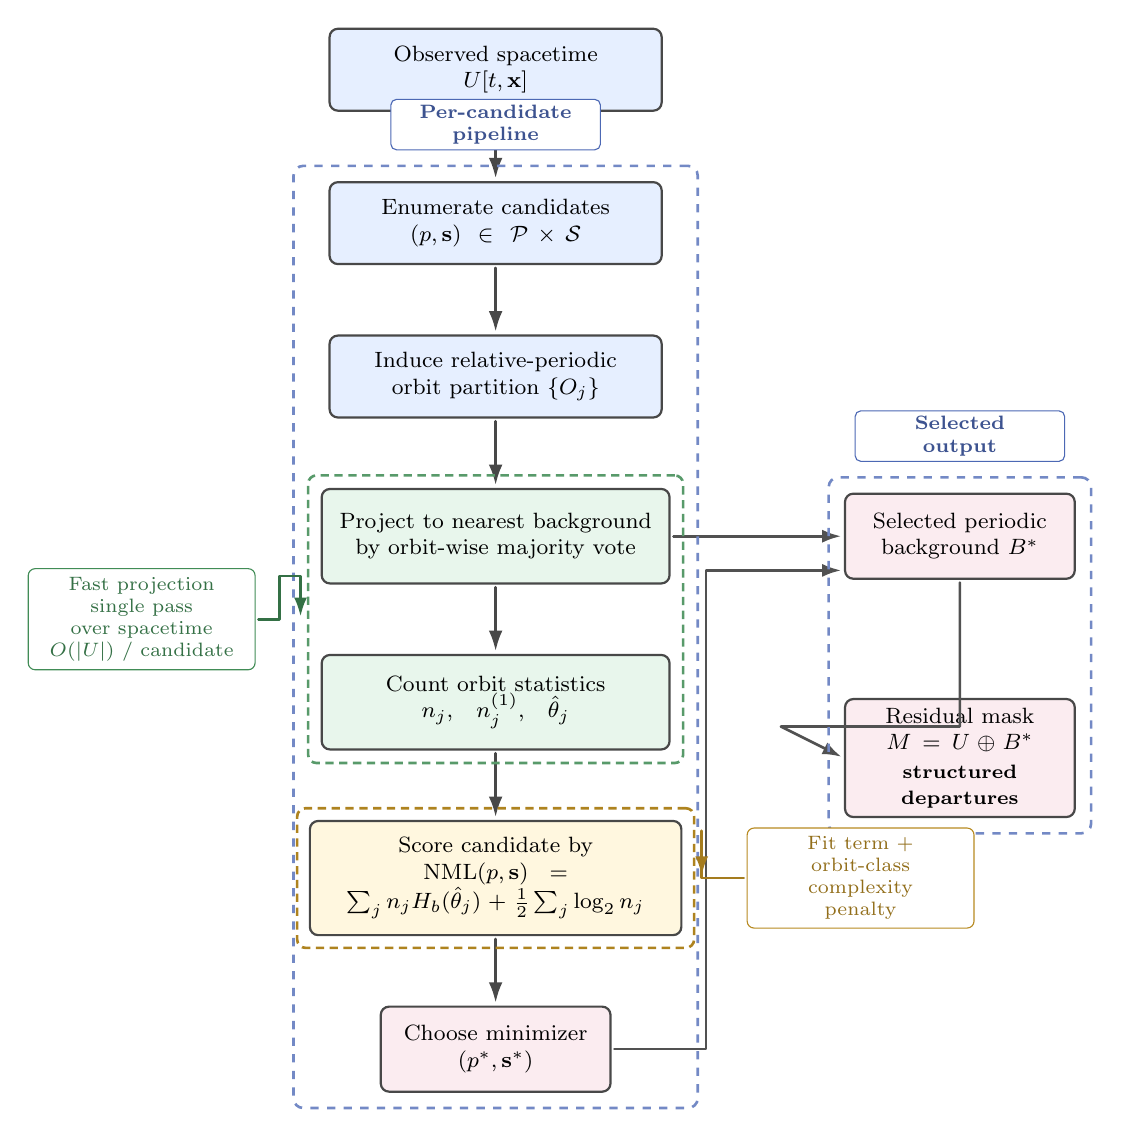
\begin{tikzpicture}[node distance=8.8mm and 9mm]
  \node[stage] (data) {Observed spacetime\\$U[t,\mathbf{x}]$};
  \node[stage, below=of data] (cand) {Enumerate candidates\\$(p,\mathbf{s}) \in \mathcal{P}\times\mathcal{S}$};
  \node[stage, below=of cand] (orbit) {Induce relative-periodic\\orbit partition $\{O_j\}$};
  \node[compute, below=of orbit] (majority) {Project to nearest background\\by orbit-wise majority vote};
  \node[compute, below=of majority] (stats) {Count orbit statistics\\$n_j,\; n_j^{(1)},\; \hat{\theta}_j$};
  \node[score, below=of stats] (scorebox) {Score candidate by\\$\mathrm{NML}(p,\mathbf{s}) = \sum_j n_j H_b(\hat{\theta}_j) + \tfrac{1}{2}\sum_j \log_2 n_j$};
  \node[output, below=of scorebox] (select) {Choose minimizer\\$(p^*,\mathbf{s}^*)$};

  \node[output, right=22mm of majority] (background) {Selected periodic\\background $B^*$};
  \node[output, below=15mm of background] (residual) {Residual mask\\$M = U \oplus B^*$\\[1pt]{\scriptsize\bfseries structured departures}};

  \draw[flow] (data.south) -- (cand.north);
  \draw[flow] (cand.south) -- (orbit.north);
  \draw[flow] (orbit.south) -- (majority.north);
  \draw[flow] (majority.south) -- (stats.north);
  \draw[flow] (stats.south) -- (scorebox.north);
  \draw[flow] (scorebox.south) -- (select.north);

  % Output routing with straight segments only.
  \coordinate (laneA) at ($(majority.east)+(10mm,0)$);
  \coordinate (laneB) at ($(select.east)+(12mm,0)$);
  \coordinate (laneC) at ($(residual.west)+(-8mm,0)$);
  \draw[sideflow] (majority.east) -- (laneA) |- (background.west);
  \draw[sideflow] (select.east) -- (laneB) |- ($(background.south west)+(0,1.2mm)$);
  \draw[sideflow] (background.south) |- ($(laneC)+(0,4mm)$) -- (residual.west);

  \node[fastscope, fit=(majority)(stats)] (fastscope) {};
  \node[scorescope, fit=(scorebox)] (scorescope) {};
  \node[mainscope, fit=(cand)(orbit)(majority)(stats)(scorebox)(select)] (loopscope) {};
  \node[mainscope, fit=(background)(residual)] (outputscope) {};

  \node[noteheader=scopeblue, anchor=south] at ($(loopscope.north)+(0,1.8mm)$) {Per-candidate\\pipeline};
  \node[noteheader=scopeblue, anchor=south] at ($(outputscope.north)+(0,1.8mm)$) {Selected\\output};

  \node[noteclaim=scopegreen, anchor=east] (fastnote) at ($(fastscope.west)+(-6.5mm,0)$) {Fast projection\\single pass over spacetime\\$O(|U|)$ / candidate};
  \node[noteclaim=scopegold, anchor=west] (scorenote) at ($(scorescope.east)+(6.5mm,0)$) {Fit term +\\orbit-class complexity\\penalty};

  \coordinate (fastscopeattach) at ($(fastscope.west)+(-0.8mm,0)$);
  \coordinate (scorescopeattach) at ($(scorescope.east)+(0.8mm,0)$);
  \draw[sideflow, draw=scopegreen!80!black] (fastnote.east) -- ++(3mm,0) |- ($(fastscopeattach)+(0,5.5mm)$) -- (fastscopeattach);
  \draw[sideflow, draw=scopegold!90!black] (scorenote.west) -- ++(-3mm,0) -| ($(scorescopeattach)+(0,6mm)$) -- (scorescopeattach);
\end{tikzpicture}
\end{document}
